\section{Funktionelle krav}\label{sec:funktionelle-krav}

\section{Use Case Diagram}
Nedenunder ses der et use case diagram lavet ud fra medarbejder-mål tabellen. Use case diagrammet giver et godt overblik over, hvilke cases de forskellige aktøre står for, samt kun noget af forholdet mellem aktør, system og use case \cite{visual-paradigm.com}. 

\begin{figure}[H]
    \centering
    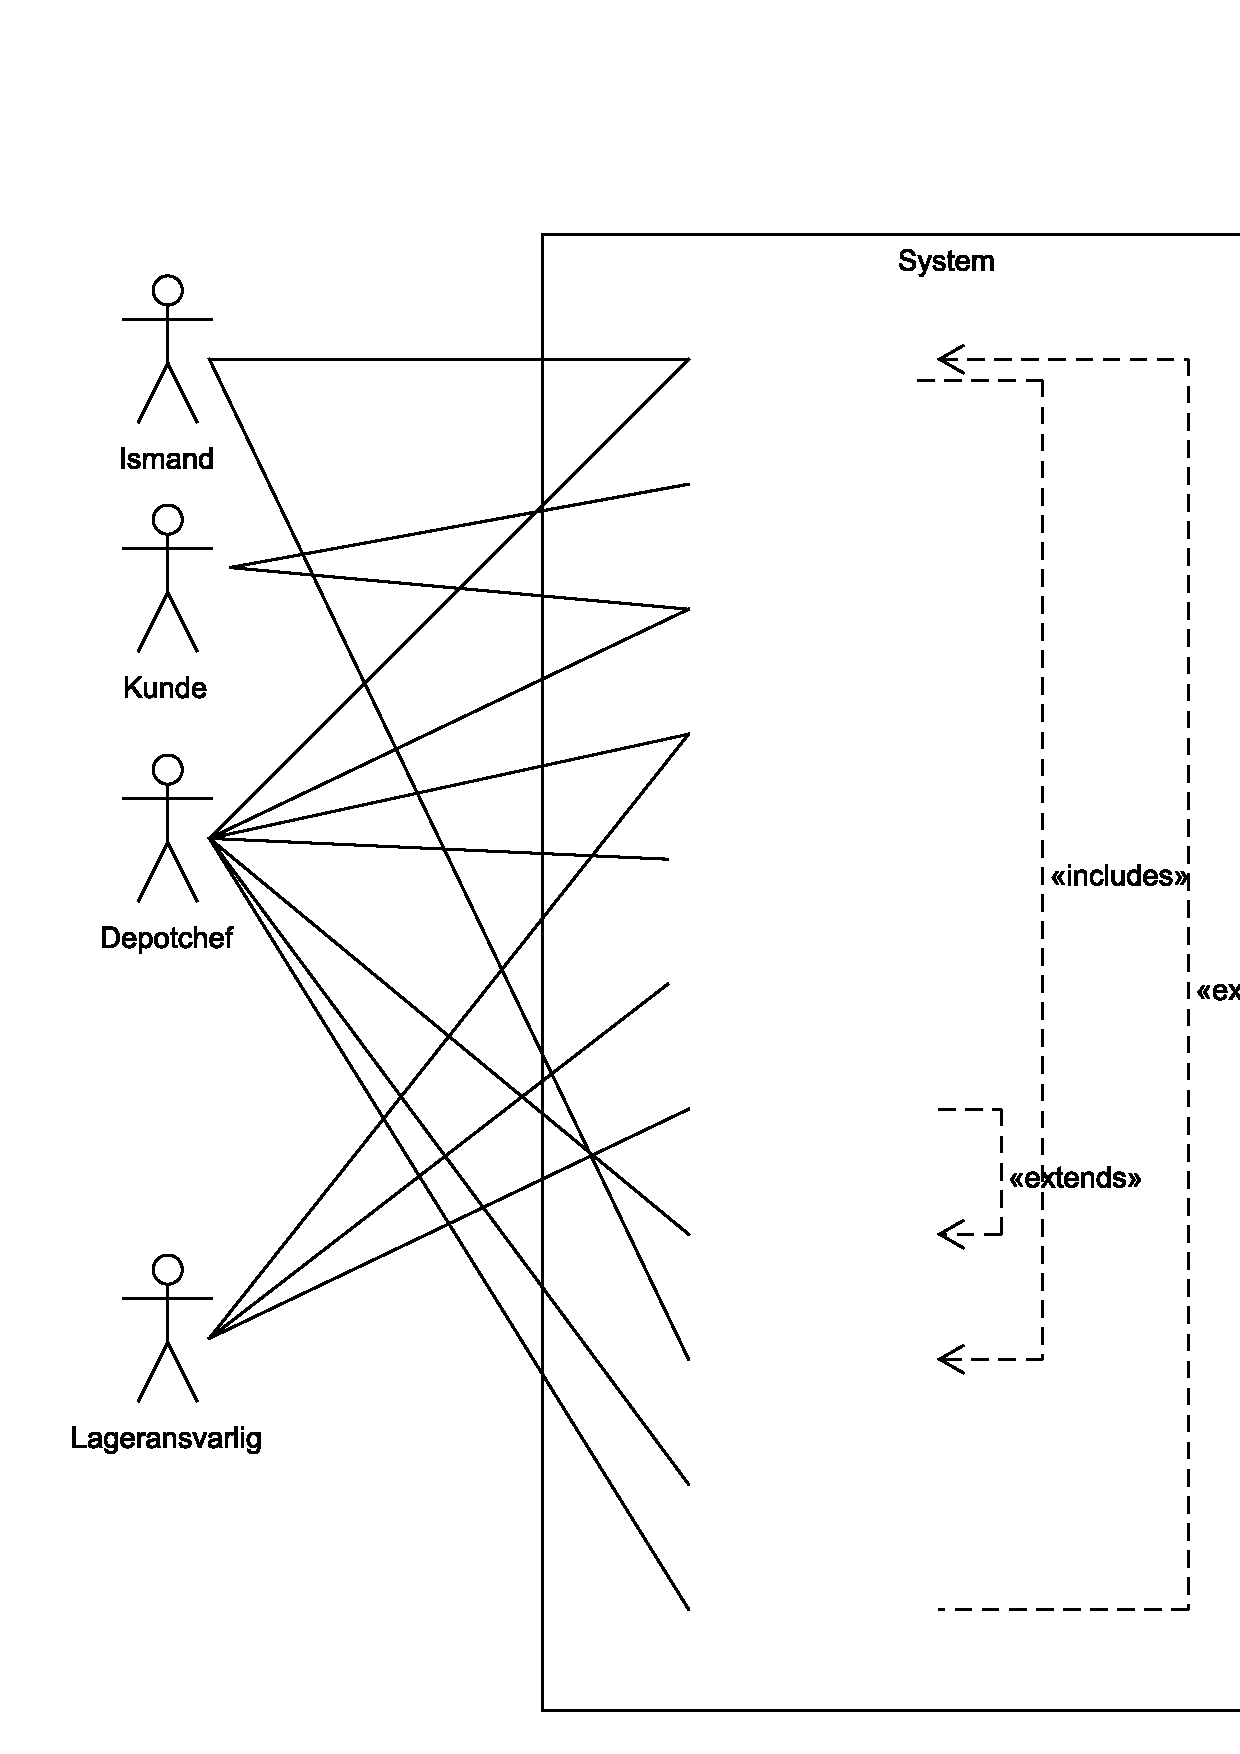
\includegraphics[width=\textwidth]{figures/Forundersøgelse/use_case_diagram.png}
    \caption{Use case diagram}
    \label{fig:use_case_diagram}
\end{figure}

Use Case diagrammet viser at depotchefen står for næsten alle opgaver i virksomheden. Depotchefen udtrykte en interesse for at kunne bruge mindre tid på de mange use cases han har i løbet af dagen, for så at kunne bruge tid på at køre salgsruter. Da det også primært er depotchefen, der står for de opgaver, som udføres i systemet, er det de Use Cases der vil blive fokuseret på.

\section{Fully Dressed}

Herunder ses Fully Dressed Use Casen ‘Automatisk lagerstyring’. Use case 'Automatisk Lagerstyring' er bygget på de tidligere use cases: 'Afskriv vare', fordi den påvirker hvor meget der er på lager. 'Optælling af isbil', som er manuelt arbejde og vil nemt kunne erstattes med automatisk optælling. 'Bestil varer', dette ville gå hånd i hånd med automatisk optælling af bilen. Og til sidst use case 'Modtag varer', fordi systemet skal opdateres med de nye varer der kommer på lager. 

De alternative flows beskrevet i diagrammet er fundet gennem en diskussion, hvor mulige fejl eller forhindringer kan opstå under flowet af handlinger. De alternative flows beskriver, hvordan et system kan fejle undervejs, hvad der er nødvendigt at være forberedt på, og hvordan disse alternative flows kan behandles så systemet ikke stopper, men kan fortsætte Use Casen til ende. Sker det at systemet eller kunden ikke opfører sig som forventet, skal de mulige udfald udtænkes, og sådanne scenarier skal kunne behandles af systemet så vidt muligt.


\begin{longtable}{ |p{120pt}|p{120pt}|p{120pt}| }
    \hline
    \textbf{Use case navn} & Automatisk lagerstyring & \\
    \hline
    \textbf{Aktør} & Depotchefen & \\
    \hline
    \textbf{Præbetingelser} & Et lager med en addresse, penge til at bestille, lagerbeholding fysisk er det samme som i systemet og en smule salgsdata & \\
    \hline
    \textbf{Postbetingelser} & Et lager tilpas fyldt med is & \\
    \hline
    \textbf{Frekvens} & 1 gang om dagen & \\
    \hline
    \textbf{Main Success Scenario} (Flow of events) & \textbf{Aktørhandling} & \textbf{Systemsvar} \\
    \hline
    & 1. Aktøren trykker på "Vis salgsstatistik" & 2. Viser salgsstatistik \\
    \hline
    & 3. Klikker på "generer lagerplan" & 4. Fil dialogboks omkring hvor bestillingsplanen skal gemmes, sendes automatisk til plan-fanen \\
    \hline
    & 5. Klikker "Åben plan" & 6. Viser bestillingsplanen med mulighed for at kunne rette i den estimerede bestillingsplan. \\
    \hline
    & 7. Klikker "Opret bestilling" & 8. Opretter en bestilling af varer ud fra bestillingsplanen. \\
    \hline
    & 9. Efter nogle dage registreres de ankomne varer i systemet & 10. Lagerstatus opdateret. \\
    \textbf{Alternative flows} & 5a. Aktøren vil gerne modificere planen, og gør det i plan-fanen & \\
    \hline
\end{longtable}

\begin{longtable}{ |p{120pt}|p{120pt}|p{120pt}| }
    \hline
    \textbf{Use case navn} & Automatisk bogføring & \\
    \hline
    \textbf{Aktør} & Depotchefen & \\
    \hline
    \textbf{Præbetingelser} & ingen & \\
    \hline
    \textbf{Postbetingelser} & bogføring er automatisk færdiggjort i et excel ark & \\
    \hline
    \textbf{Frekvens} & 1 gang om dagen & \\
    \hline
    \textbf{Main Success Scenario} (Flow of events) & \textbf{Aktørhandling} & \textbf{Systemsvar} \\
    \hline
    & 1. klikker "export bogføring" & 2. systemet exporter en excel fil med bogføring \\
    \hline
\end{longtable}